\documentclass{exam}
\renewcommand{\thequestion}{Q.\arabic{question}}%
\usepackage[margin=1in]{geometry}
\usepackage{amsmath,amsfonts,amssymb}
\usepackage{multicol}
\usepackage{graphicx}
%\usepackage{nopageno}

\begin{document}
	
	
\begin{center}
		\begin{minipage}{0.1\textwidth}
			
\includegraphics[scale=0.1]{vcet-logo.jpeg}
		\end{minipage}
		\hfill 
		\begin{minipage}{0.85\textwidth}
			\textbf{\Large \textbf{\begin{center}  Vidyavardhini's College of Engineering and Technology, Vasai (West) \end{center} }}
		\end{minipage}
		
		\vspace{0.3cm}
		\textbf{\large \underline{First Year Engineering}} \\
		\vspace{0.3cm}
		\textbf{\large Academic Year: 2024-2025} \\
		\vspace{0.3cm}
		\textbf{\large Solution to the prevous year questions papers [2017 $-$ 2024] \footnote{This document has been compiled solely for the benefit of students. Permission is granted to use and distribute this material strictly for non-commercial purposes. Some content has been referenced from various academic sources, and all rights remain with the original copyright holders.} }\\
	\end{center}

\noindent
\textbf{Subject: BSC102/AP} \hfill { \textbf{Date: 20/11/2024} }\\ 
%\textbf{Max Marks: 10} \hfill { \textbf{Duration: 1 Hr} }\\
\hrule
\begin{center}
\textbf{\large Module-4: Electrodynamics } 
\end{center}
\hrule
\vspace{0.3cm}

\begin{center} \textbf{ \Large Maxwell's Equations} \end{center}

\begin{questions}
\question \textbf{ Explain Gauss’s laws for static electric and static magnetic fields in differential and integral forms. \hfil [5 Marks] [May-2022, May-2023] }
	
\textbf{Ans:}
\begin{center}
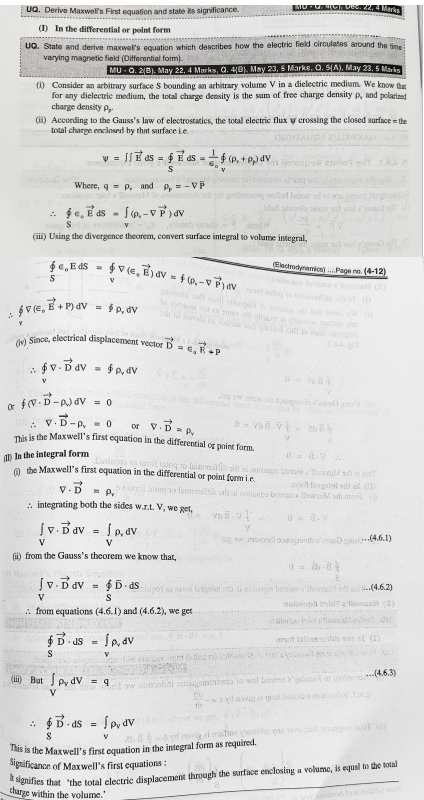
\includegraphics[scale=0.45]{Q1.png} 
\end{center}

\begin{center}
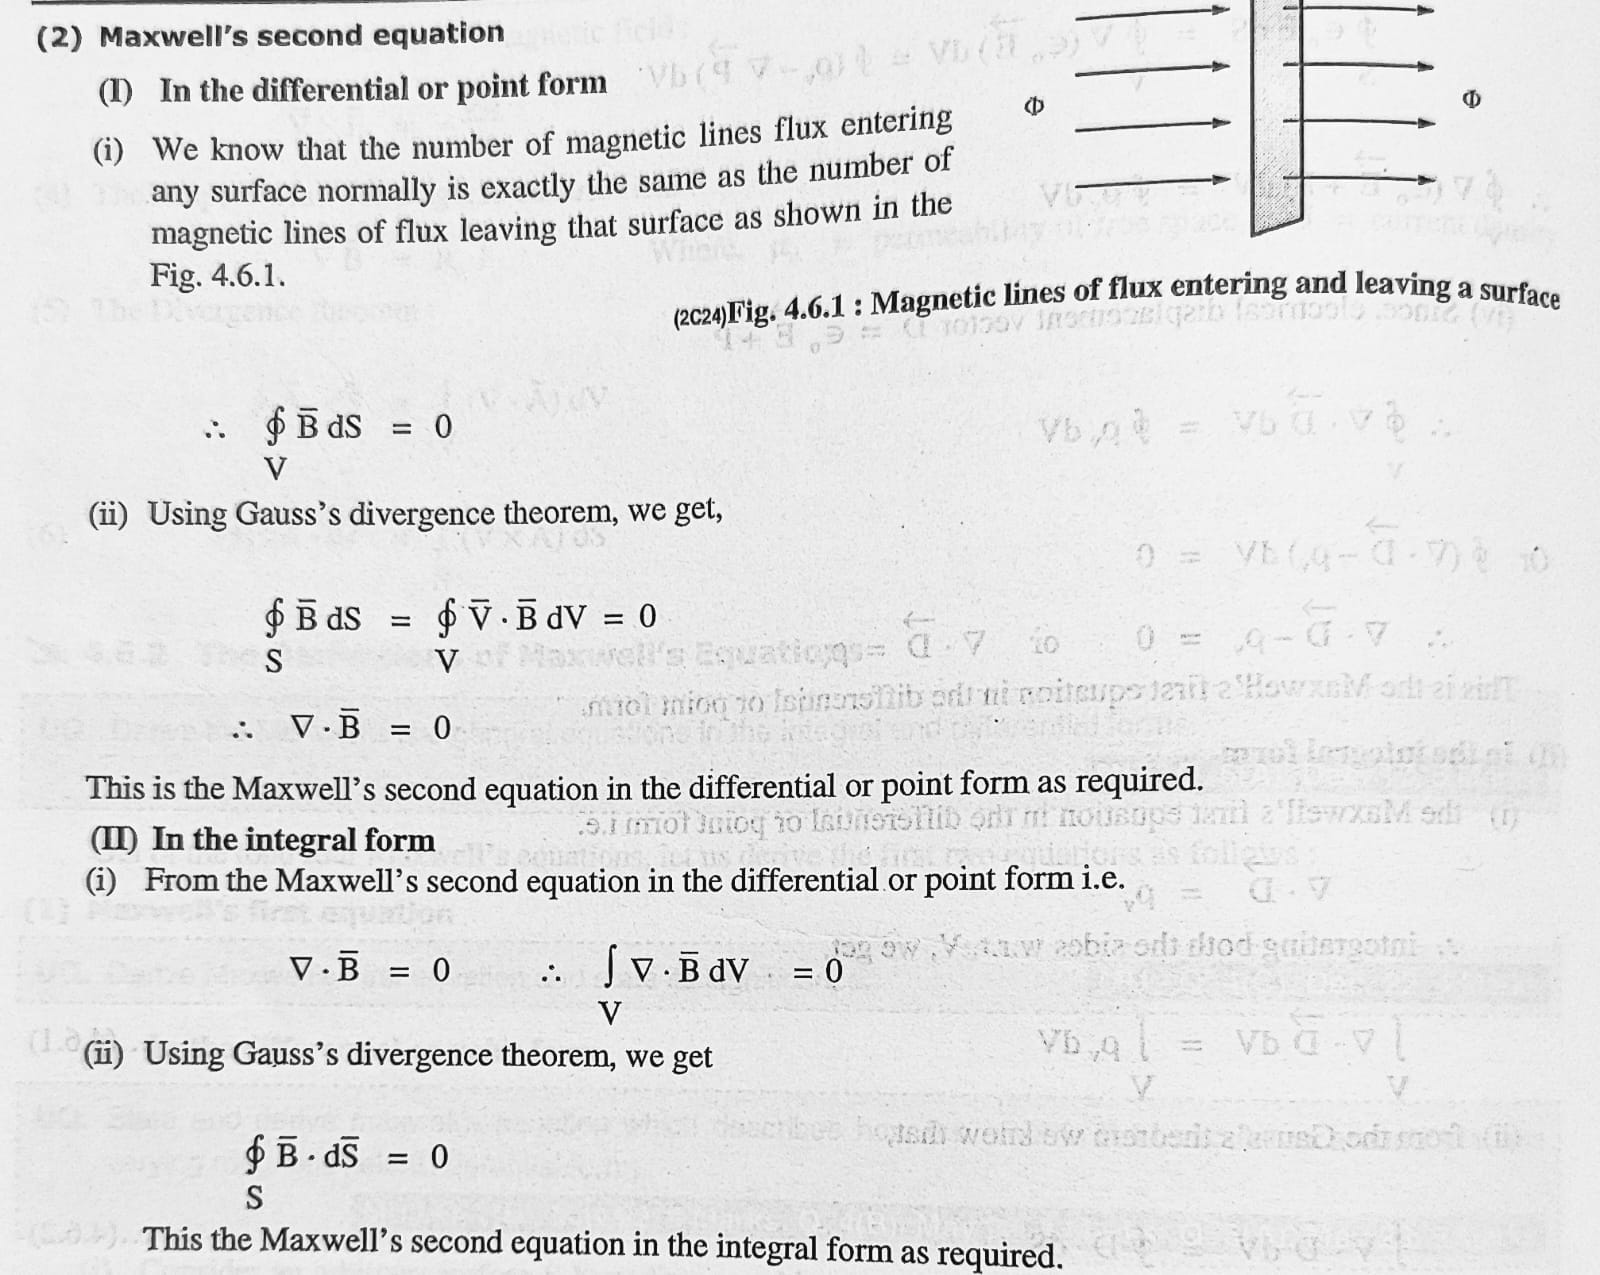
\includegraphics[scale=0.1]{Q1-3.jpeg} \\
\end{center}
	
\question \textbf{ State and derive Maxwell’s equation in differential form which describes how the electric field circulates around the time-varying magnetic field. \hfil [5 Marks] [Dec-2018, May-2022, Dec-2022] }

\textbf{Ans:}
\begin{center}
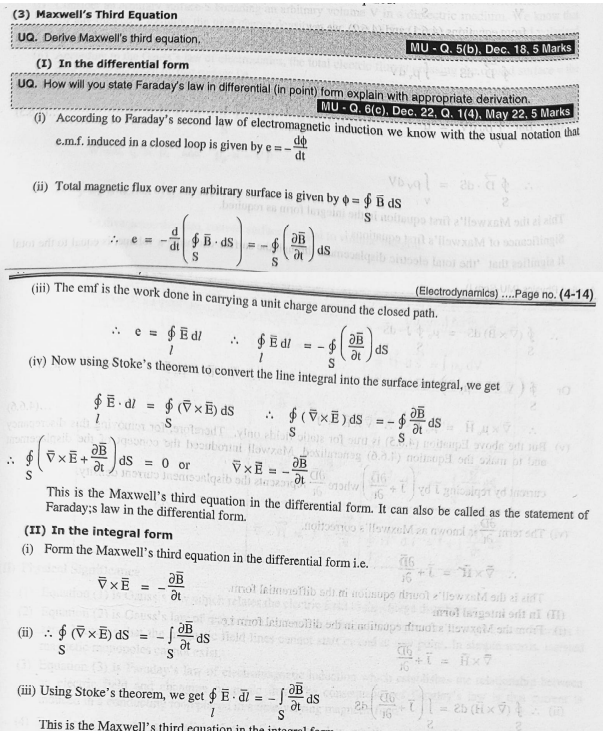
\includegraphics[scale=0.55]{Q2.png} 
\end{center}

\newpage

\question \textbf{Obtain Ampere’s circuital law for a static magnetic field in differential and integral forms.  \hfil [5 Marks] Dec-2018, May-2022, Dec-2022] }

\textbf{Ans:}
\begin{center}
	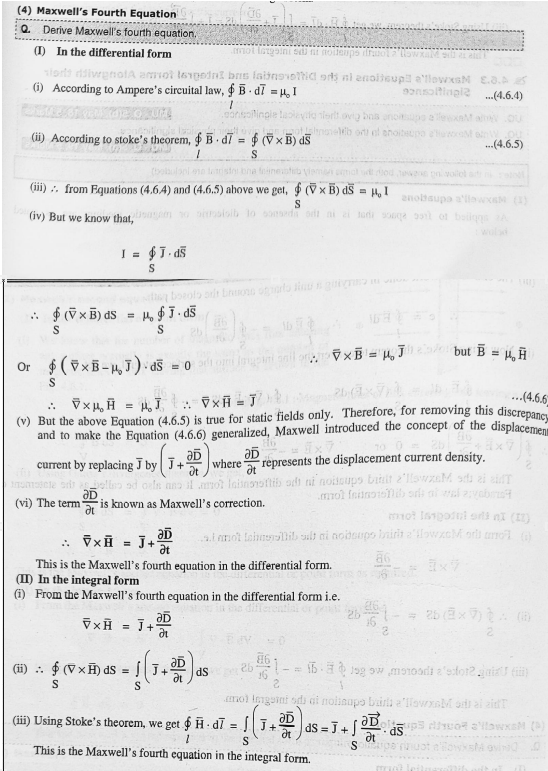
\includegraphics[scale=0.545]{Q3.png} 
\end{center}

\end{questions}

\begin{center} \textbf{ \Large Q1. Gradient, Divergence and Curl\footnote{Similar numericals based on the same concept were asked; however, only one example is presented here. As it is a numerical problem, students are encouraged to practice similar problems for better understanding.}} \end{center}

\begin{enumerate}
	
	\item[(a)]  \textbf{What are scalar and vector fields? How is a del operator expressed?   \hfil [3 Marks] [May-2019, May-2023] }
	
	\item[(b)] \textbf{ If $\phi(x,y,z) = 3x^2y - y^3z^2$, find $\nabla \phi$ at the point $(-1, -2, 1)$.  \hfil [3 Marks] [May-2019, May-2023] }
	
	\item[(c)] \textbf{ What is the divergence of a vector field? Find the divergence of a field $\mathbf{F} = xz \hat{i} + y^2 z^3 \hat{j} - xyz \hat{k}$ at a point $(3, -1, 2)$. Interpret the result you obtain.  \hfil [3 Marks] [May-2017, May-2022 Dec-2022, Dec-2023] }
	
	\item[(d)] \textbf{ Explain the term ‘curl of a vector’ and state its significance. Show that the divergence of the curl of a vector is zero.    \hfil [3 Marks] [Dec-17,May-2023, Dec-2023] }
	
\end{enumerate}

\newpage

\textbf{Ans:}
\begin{center}
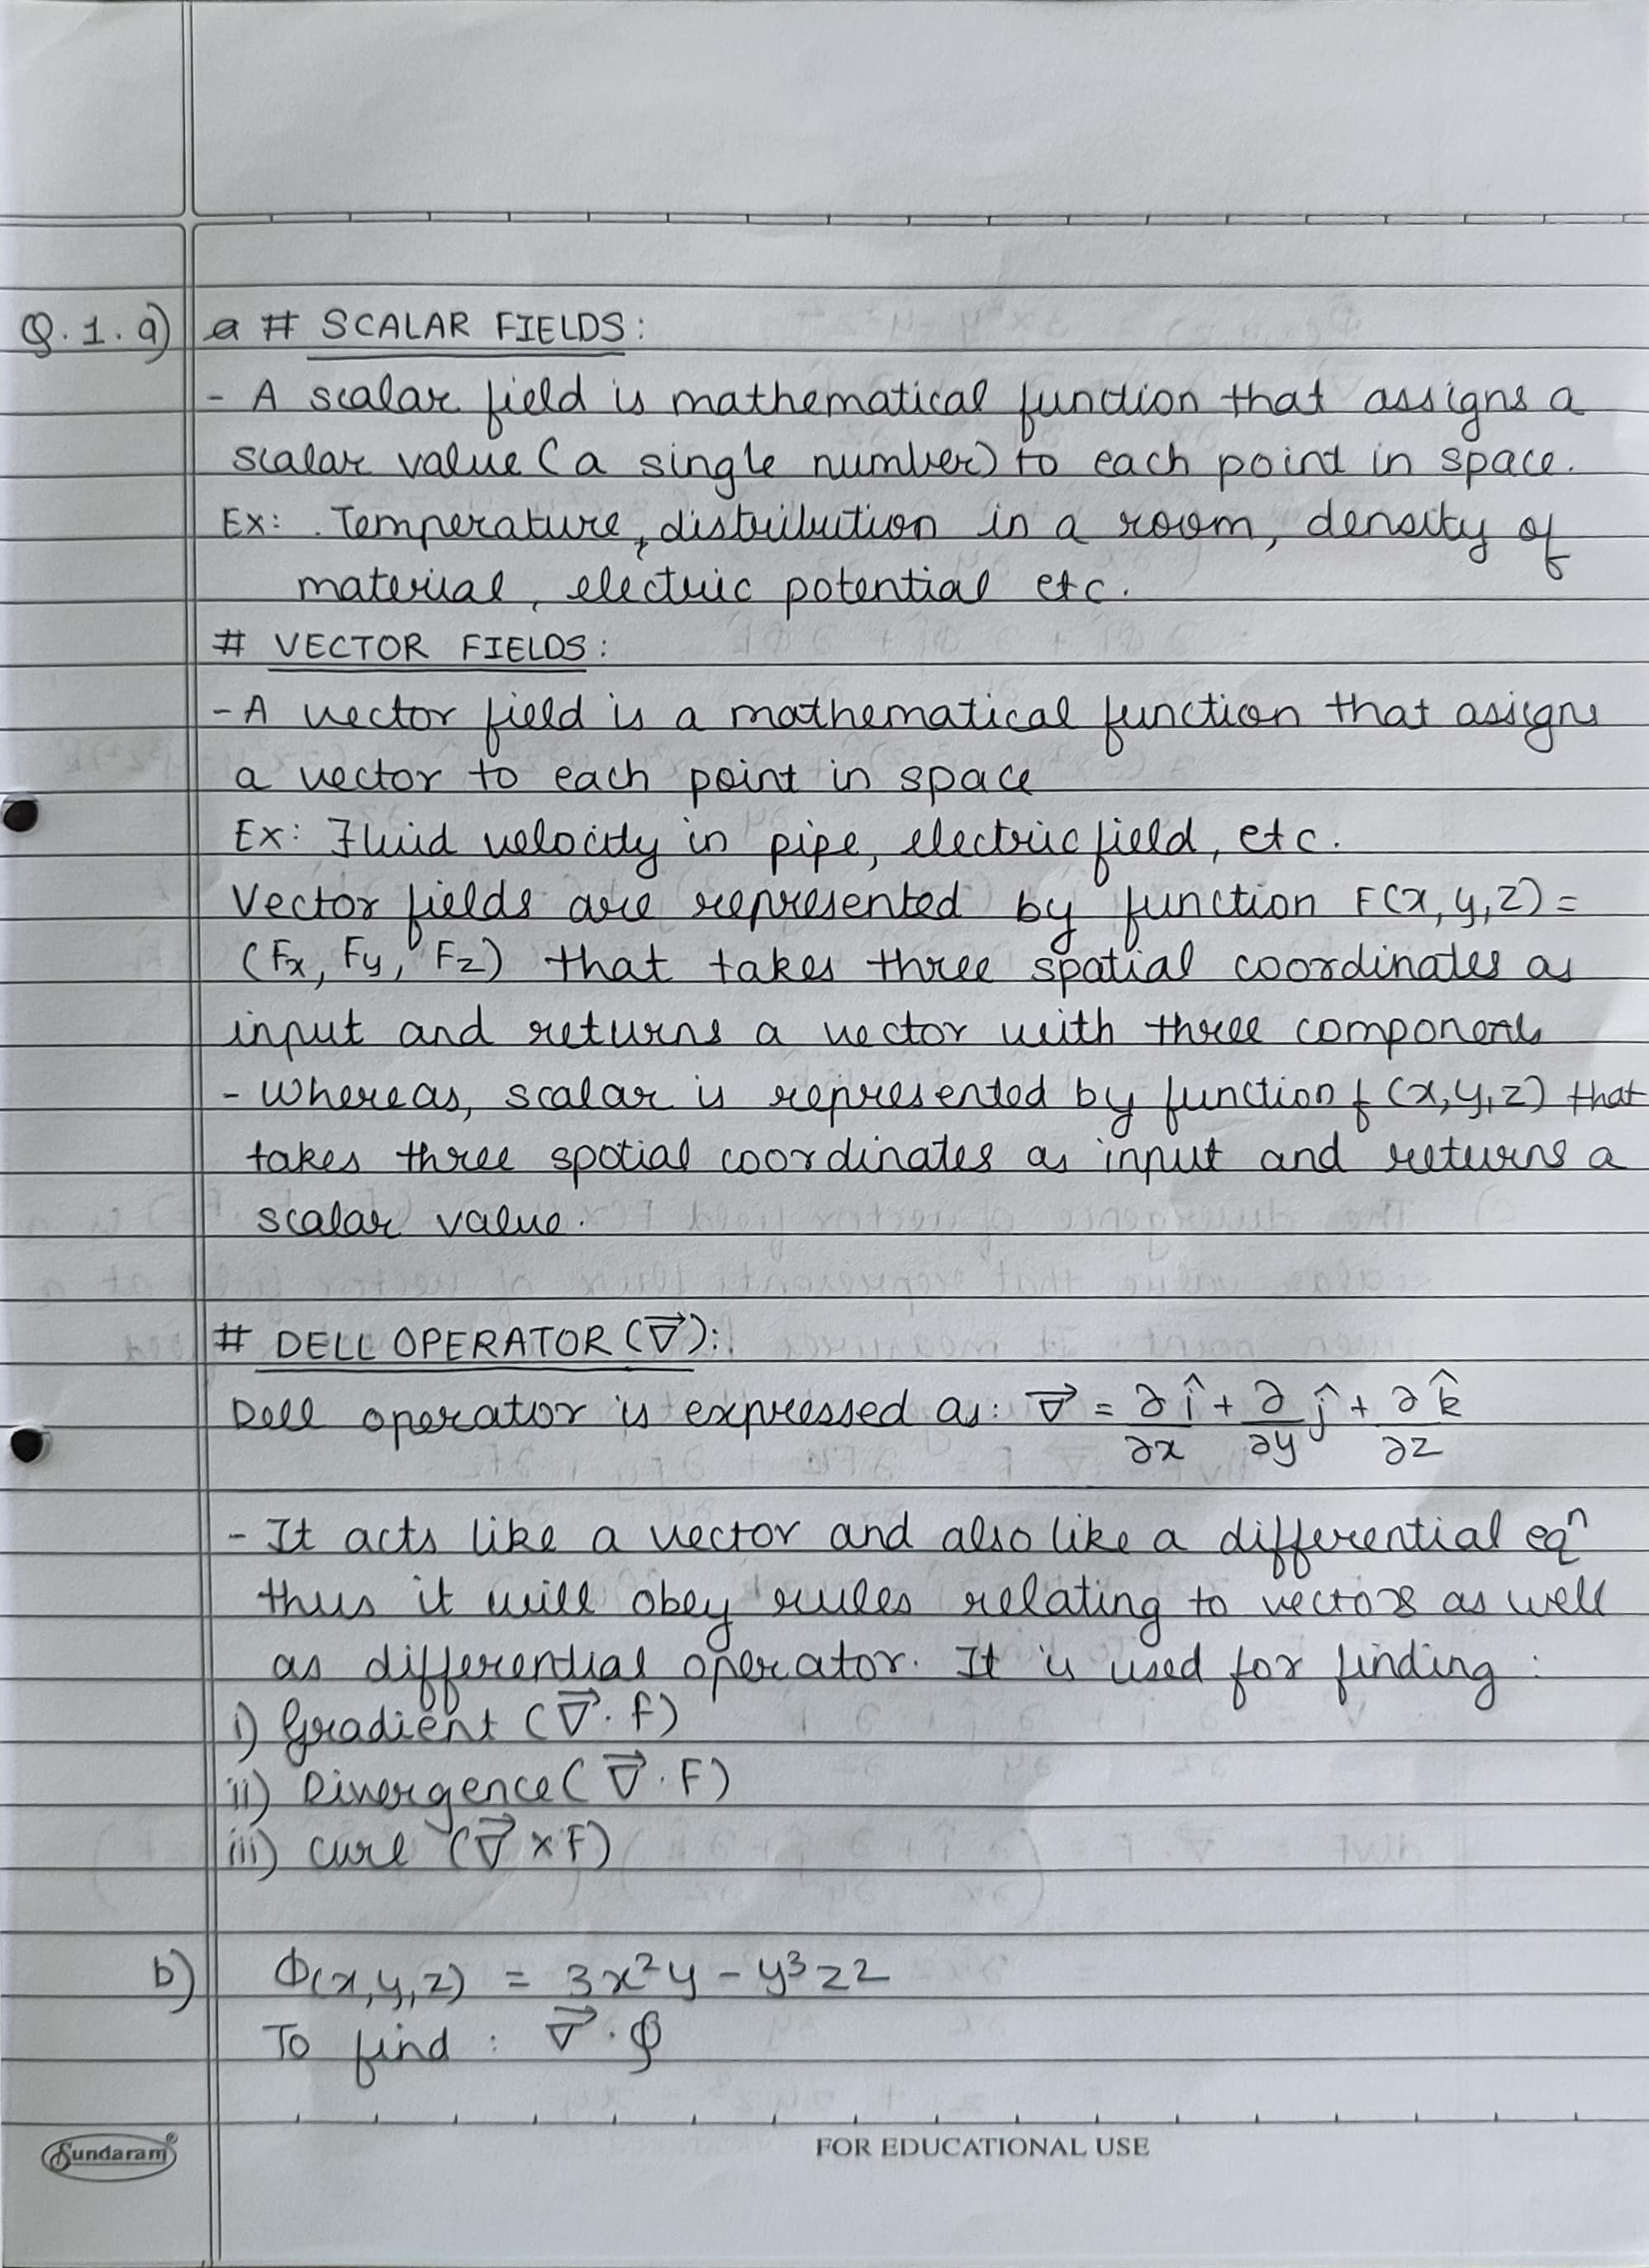
\includegraphics[scale=0.23]{1.jpeg} 
\end{center}

\newpage
\begin{center}
	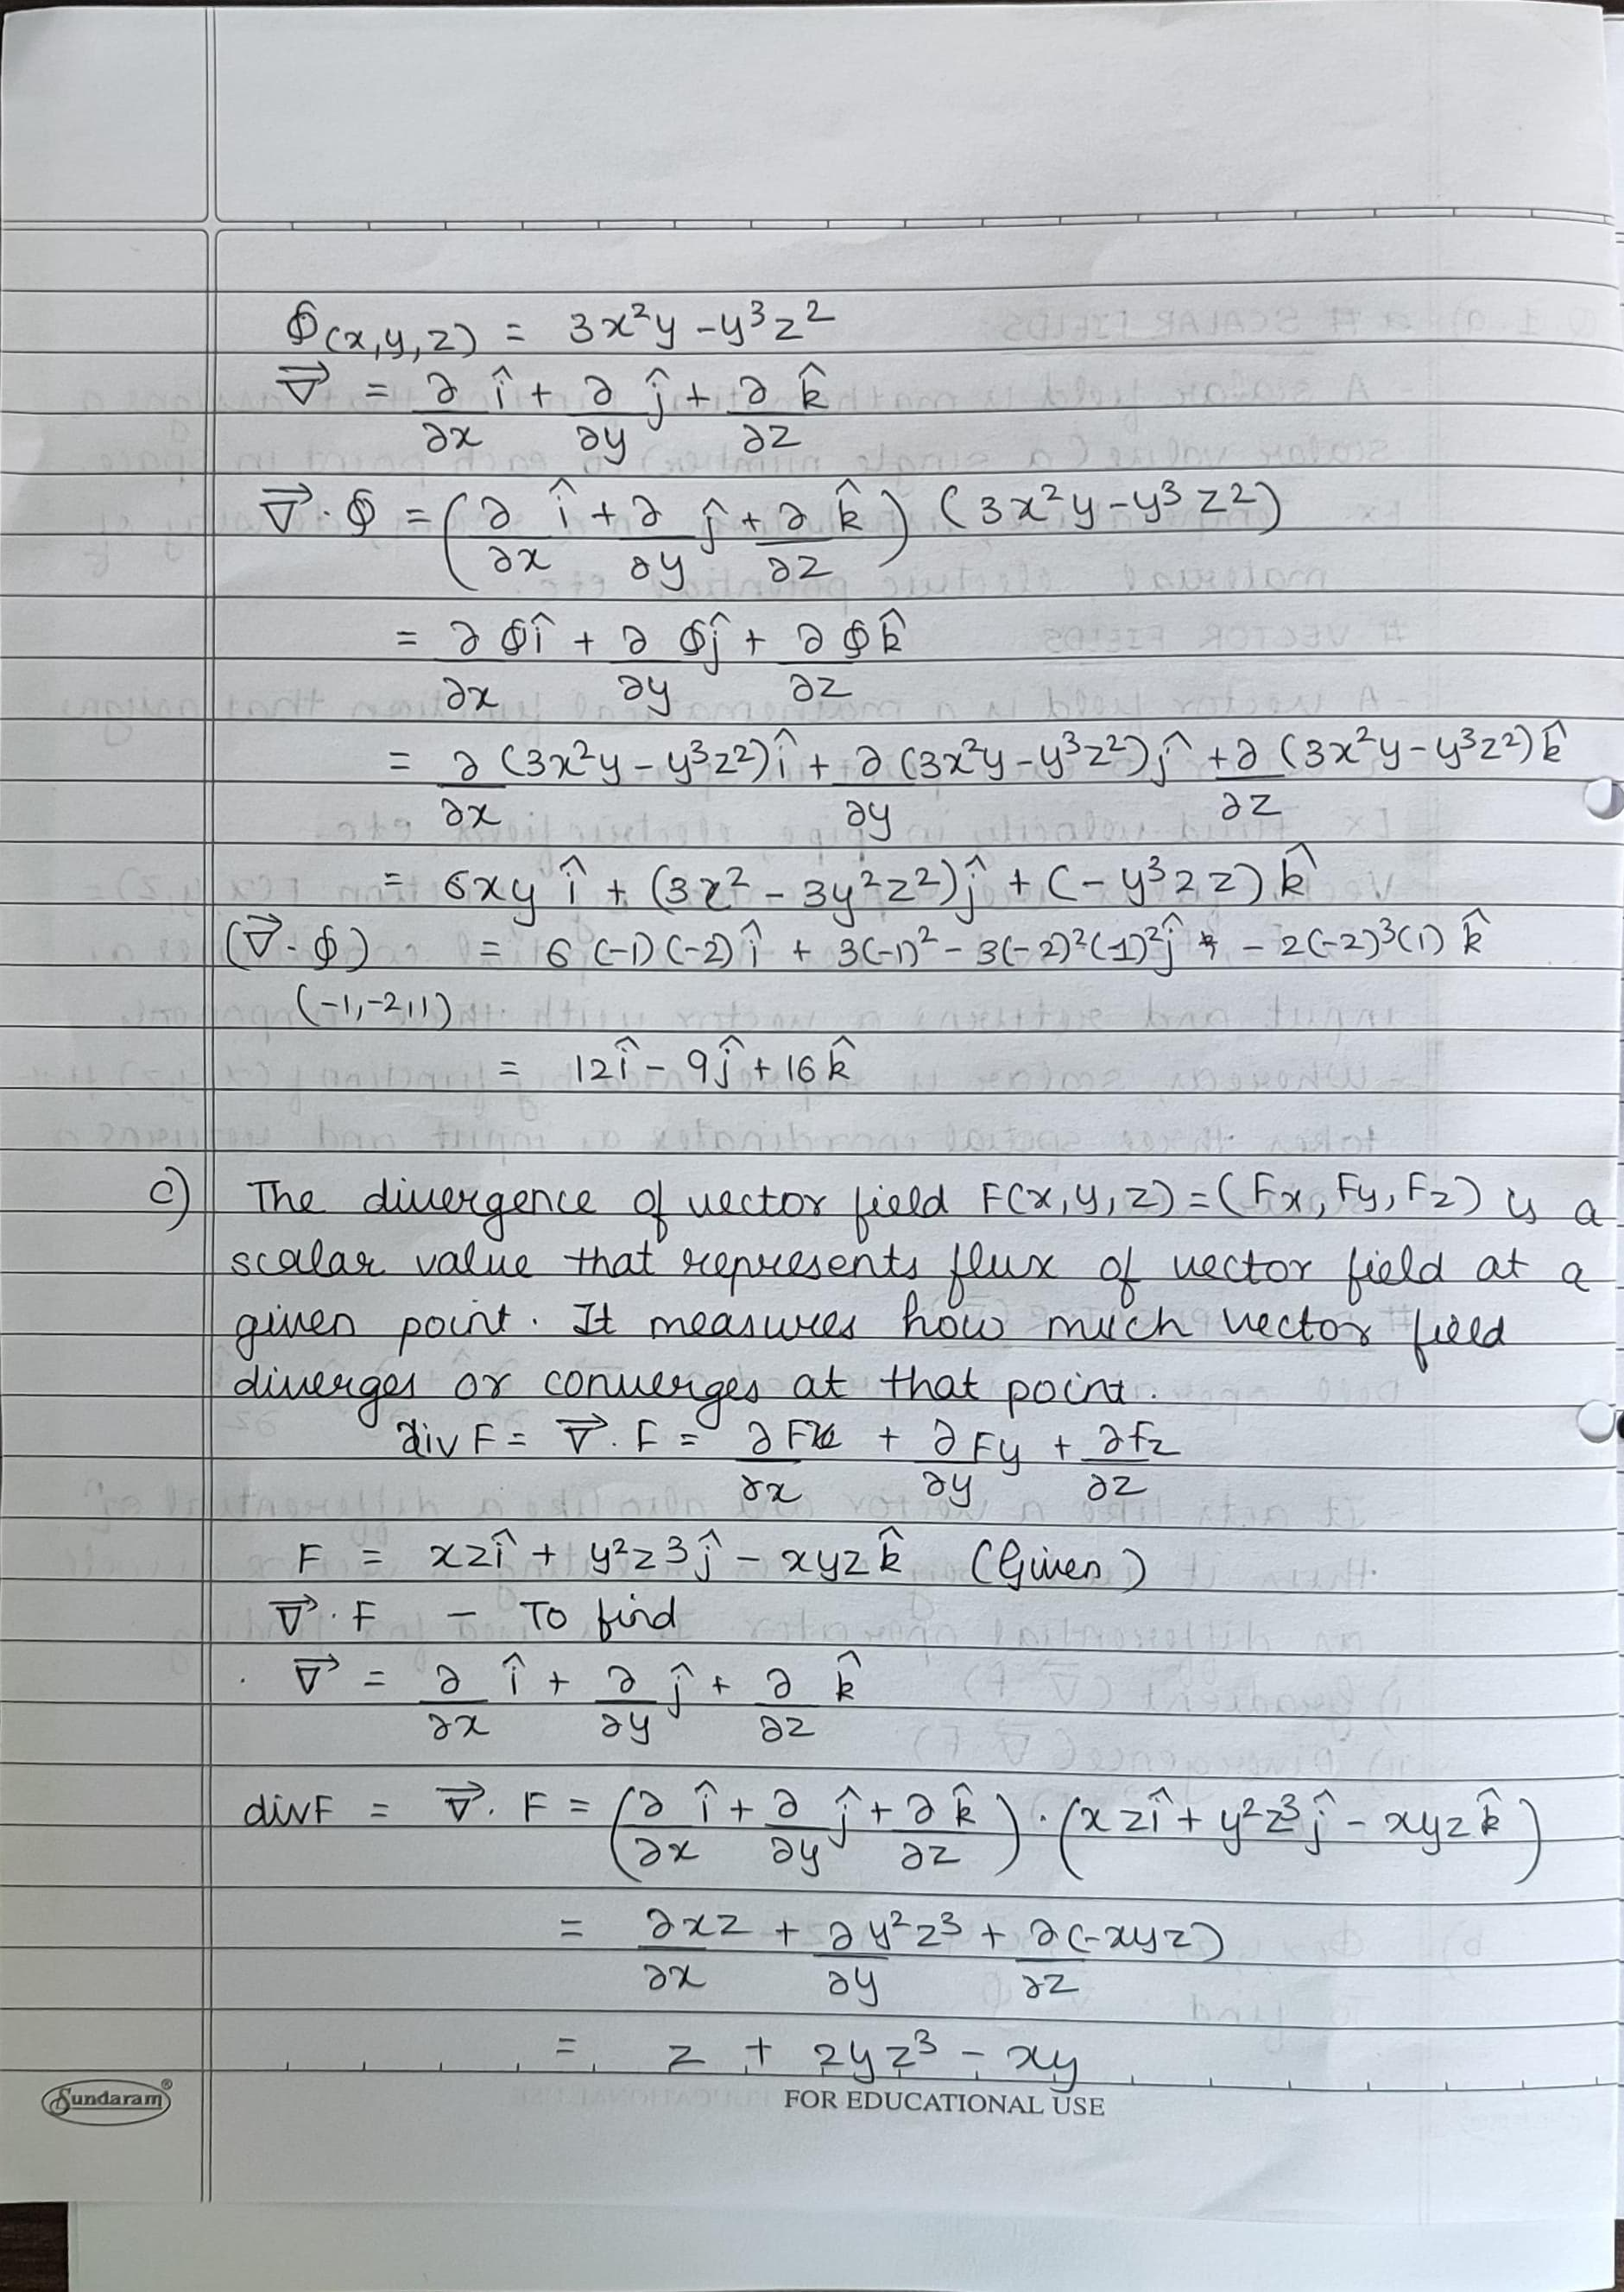
\includegraphics[scale=0.23]{2.jpeg} 
\end{center}

\newpage
\begin{center}
	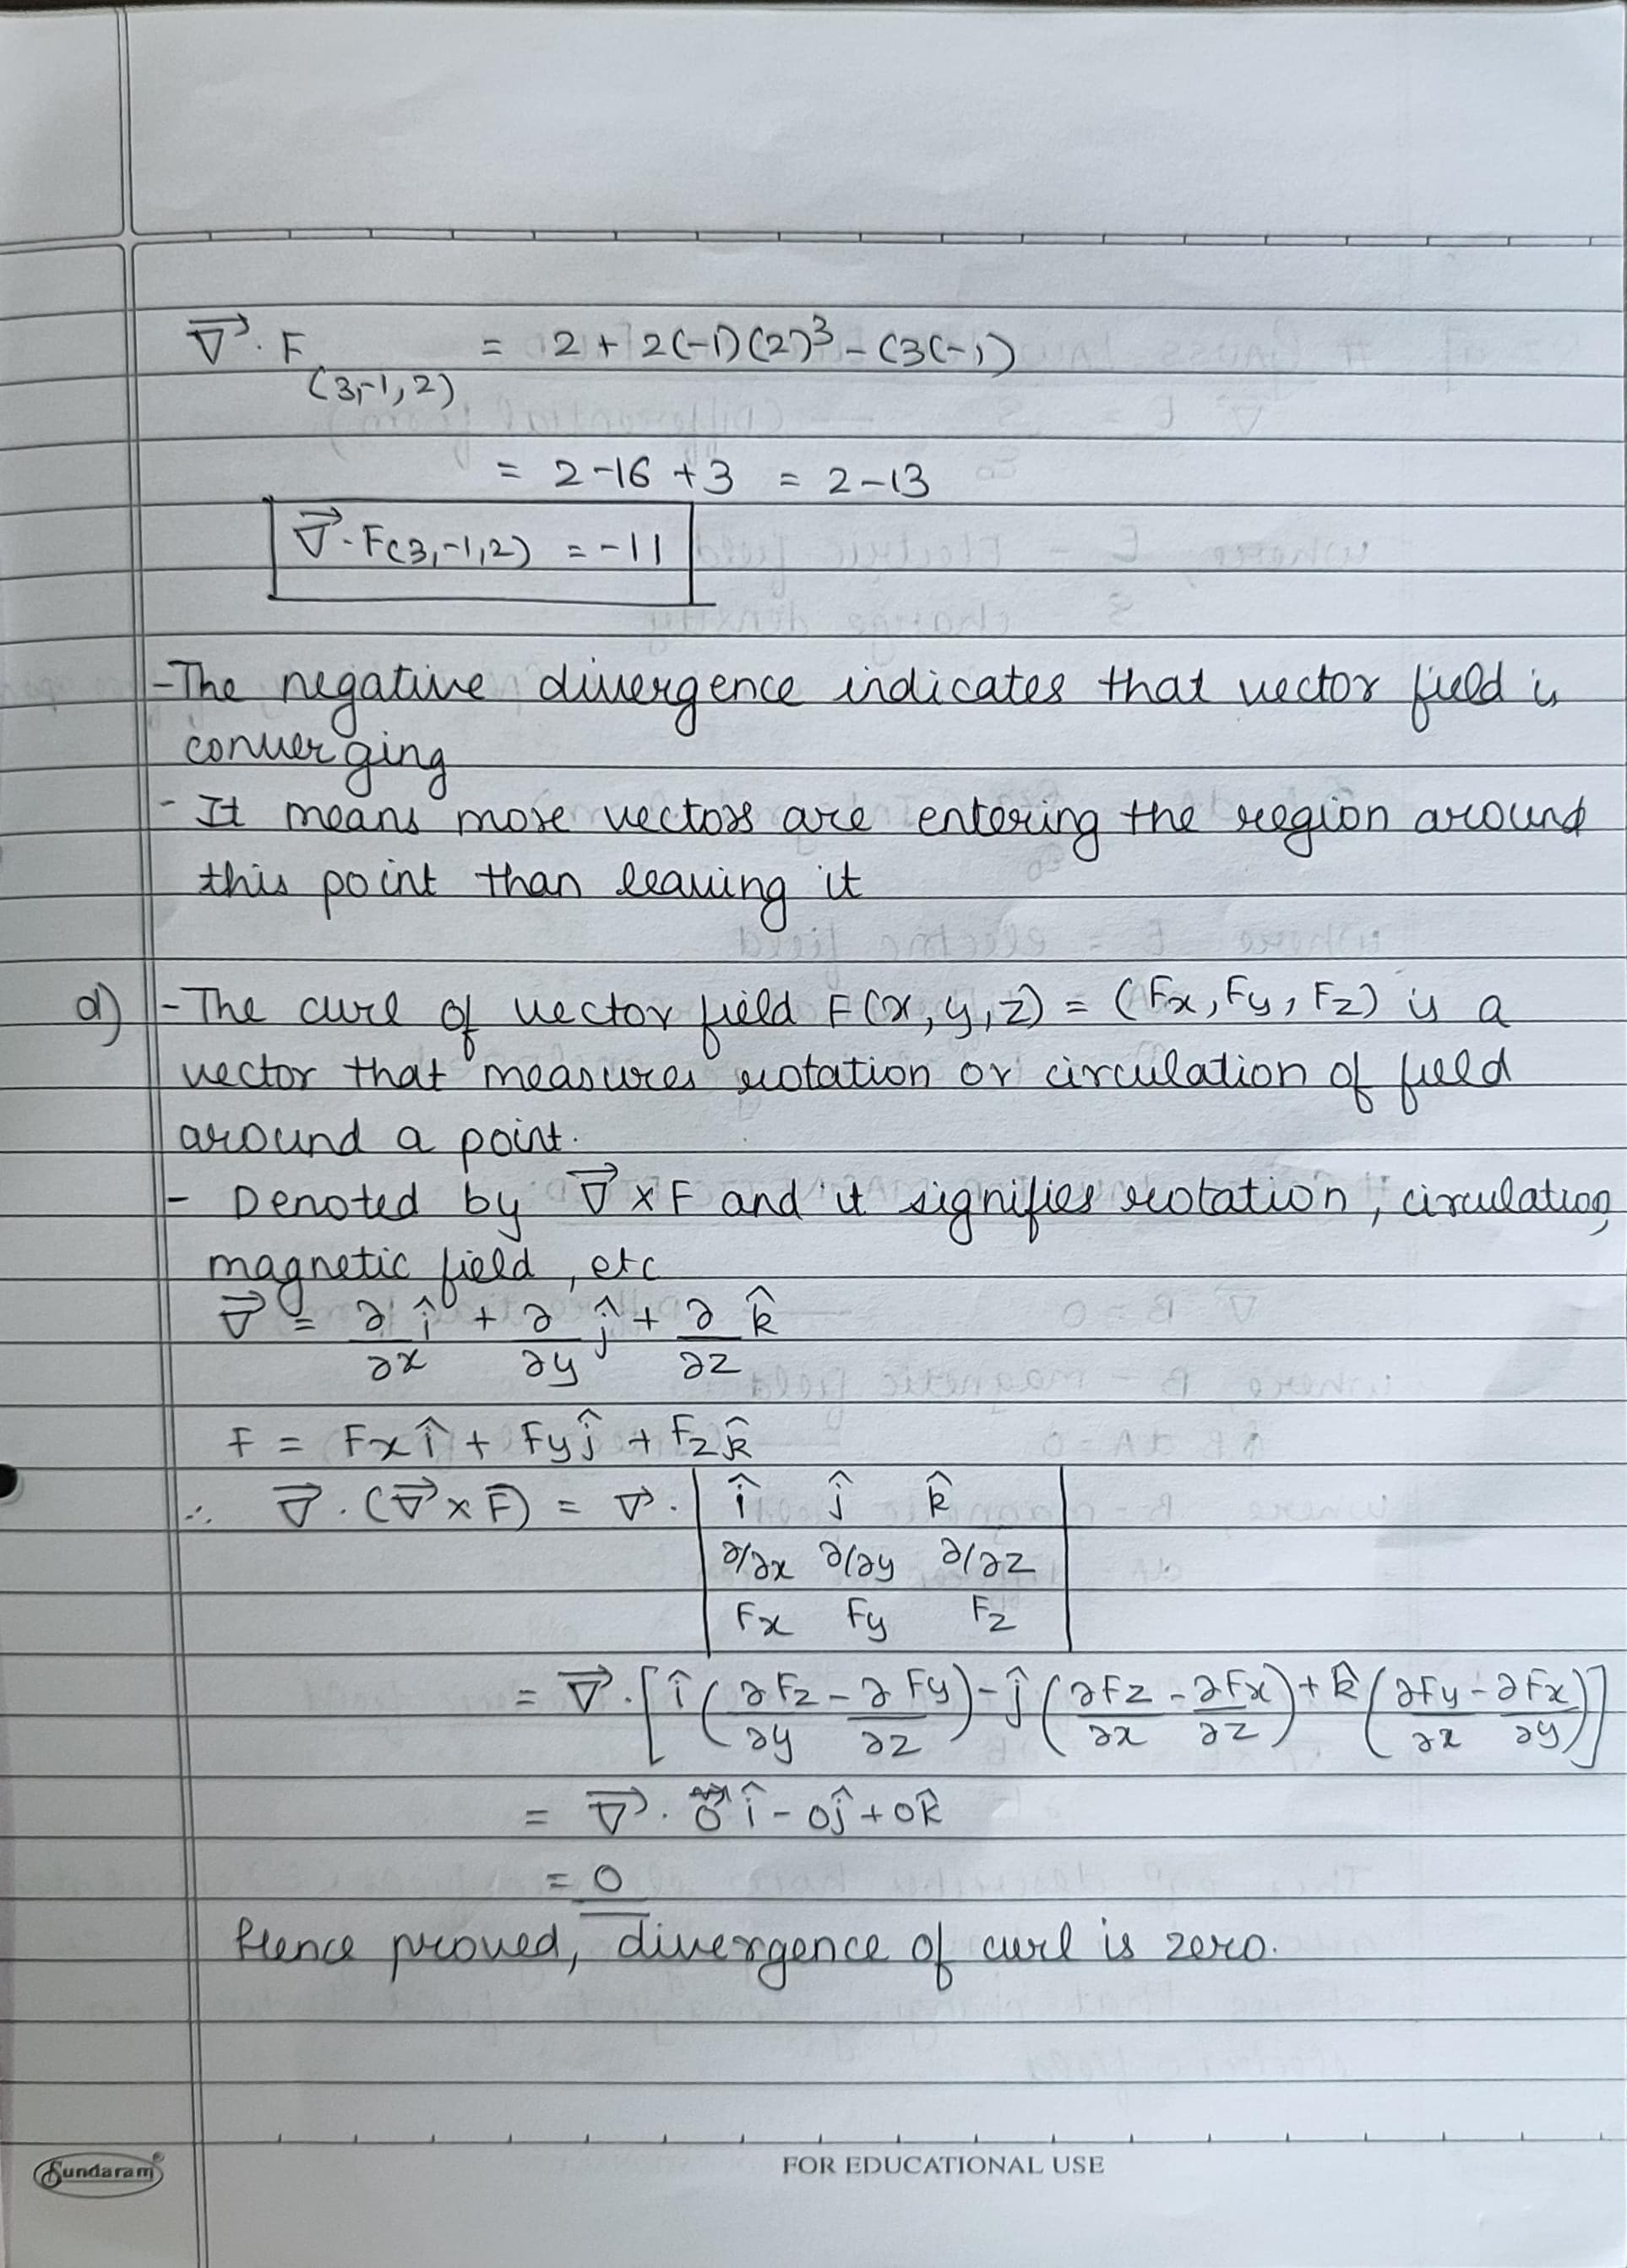
\includegraphics[scale=0.23]{3.jpeg} 
\end{center}

\vspace{0.5cm}


\vspace{0.1cm}
\noindent

	
\end{document}
